%-------------------------------------------------------------
%---------------------- Apêndices ----------------------------
%-------------------------------------------------------------

\begin{apendicesenv}
\partapendices  % Indica o início dos Apendices

\chapter{Codigo em pyhton}

\begin{figure}[h]
\caption{Tempo em horas}
 
\centering % para centralizarmos a figura
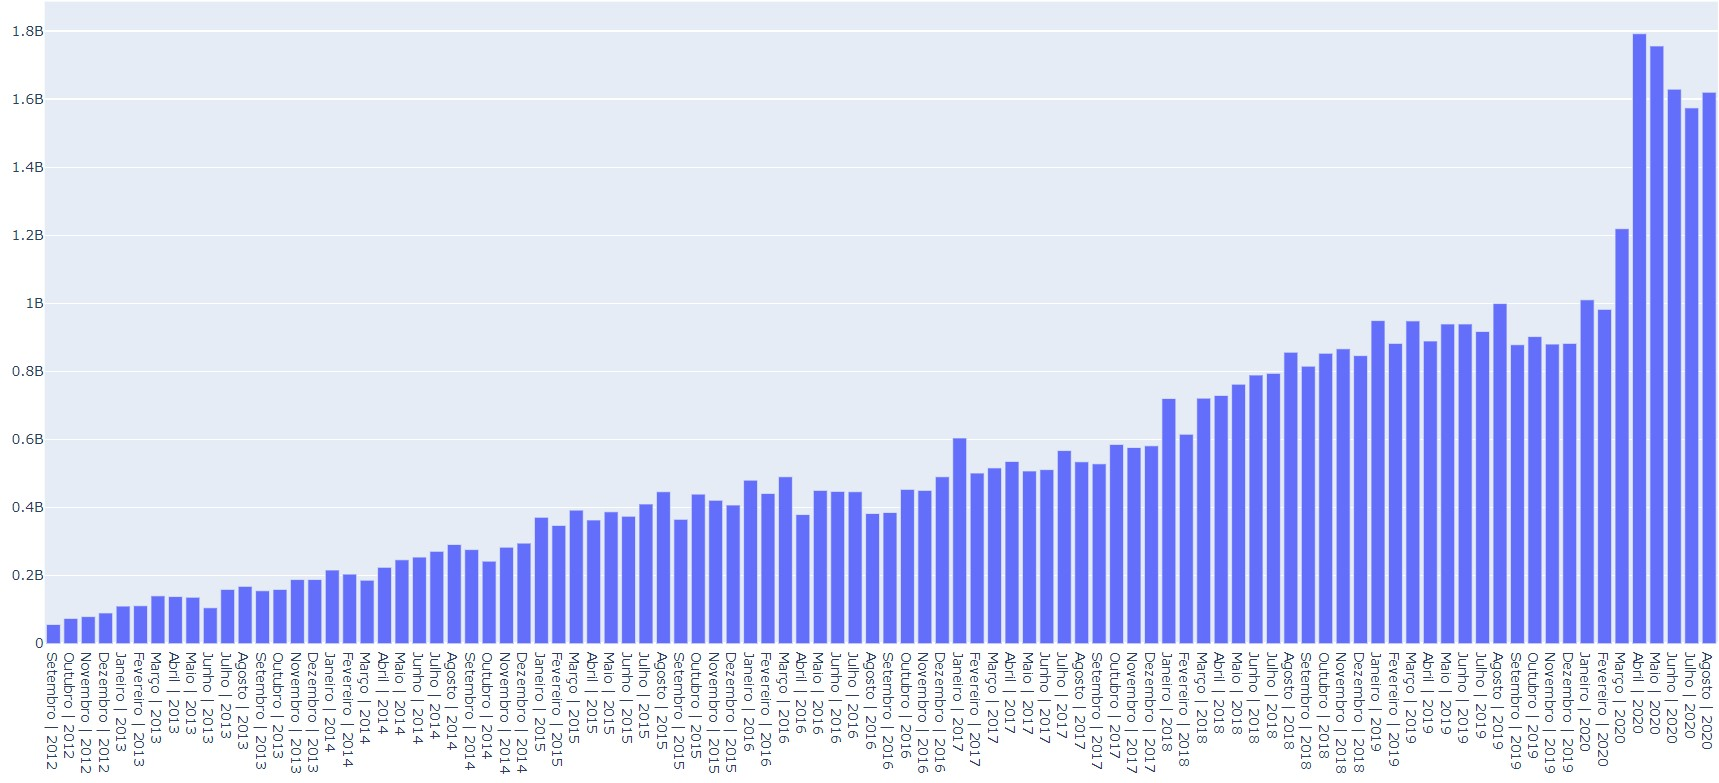
\includegraphics[width=17cm]{Figuras/Tempo_horas.jpg} % leia abaixo
\label{figura:qualquernome}
\end{figure}
Na Fig. \ref{figura:qualquernome}, Grafico em barras do tempo em horas assistido na plataforma
\begin{figure}[h]
\caption{Tempo em horas}
 
\centering % para centralizarmos a figura
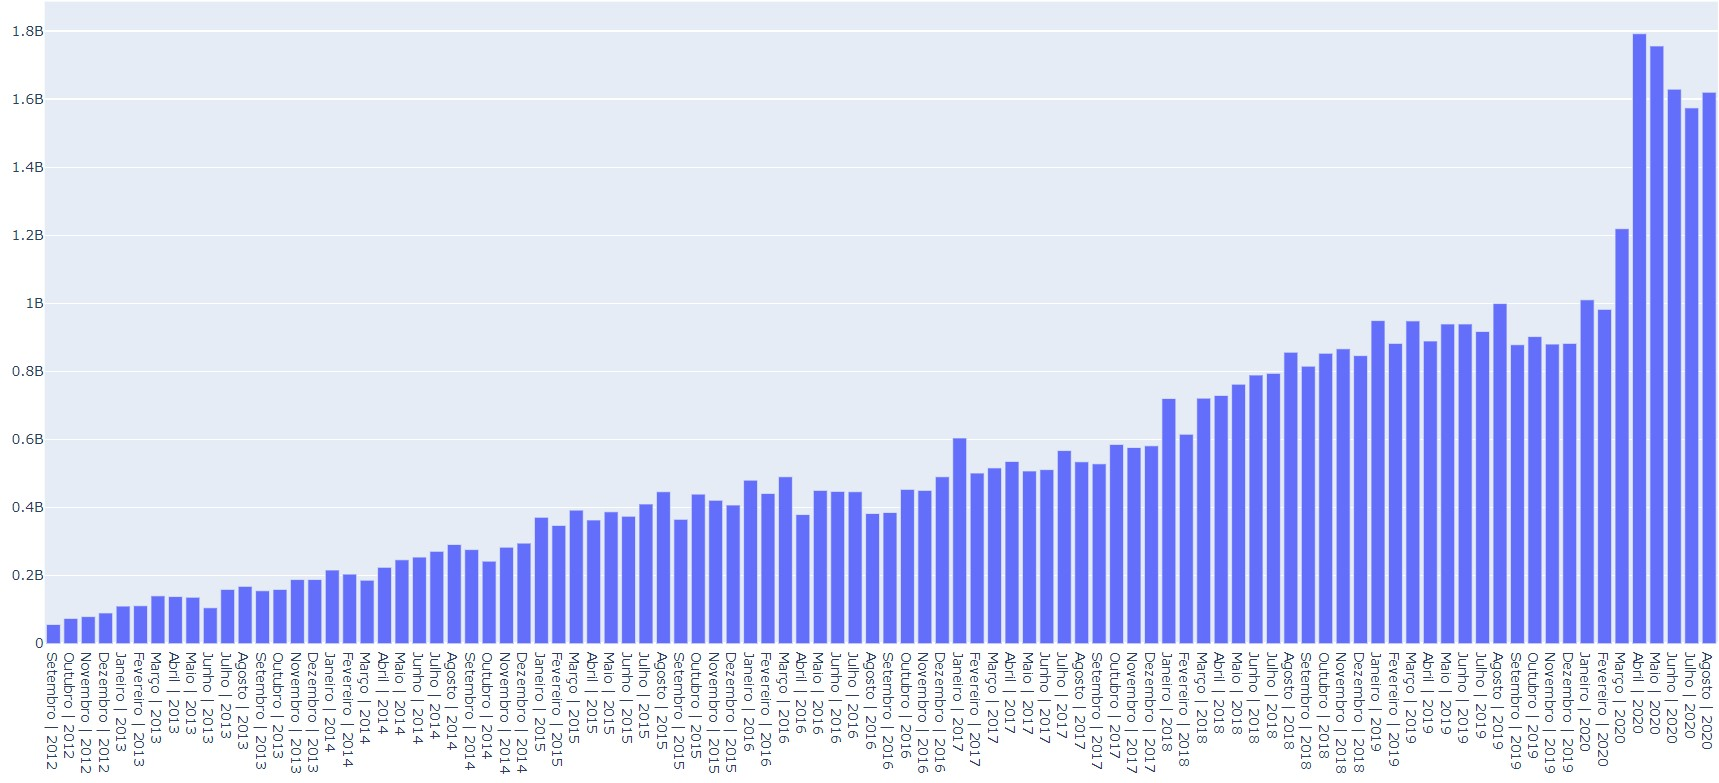
\includegraphics[width=17cm]{Figuras/Tempo_horas.jpg} % leia abaixo
\label{figura:qualquernome}
\end{figure}
Na Fig. \ref{figura:qualquernome}, Grafico em barras do tempo em horas assistido na plataforma
\begin{figure}[h]
\caption{Tempo em horas}
 
\centering % para centralizarmos a figura
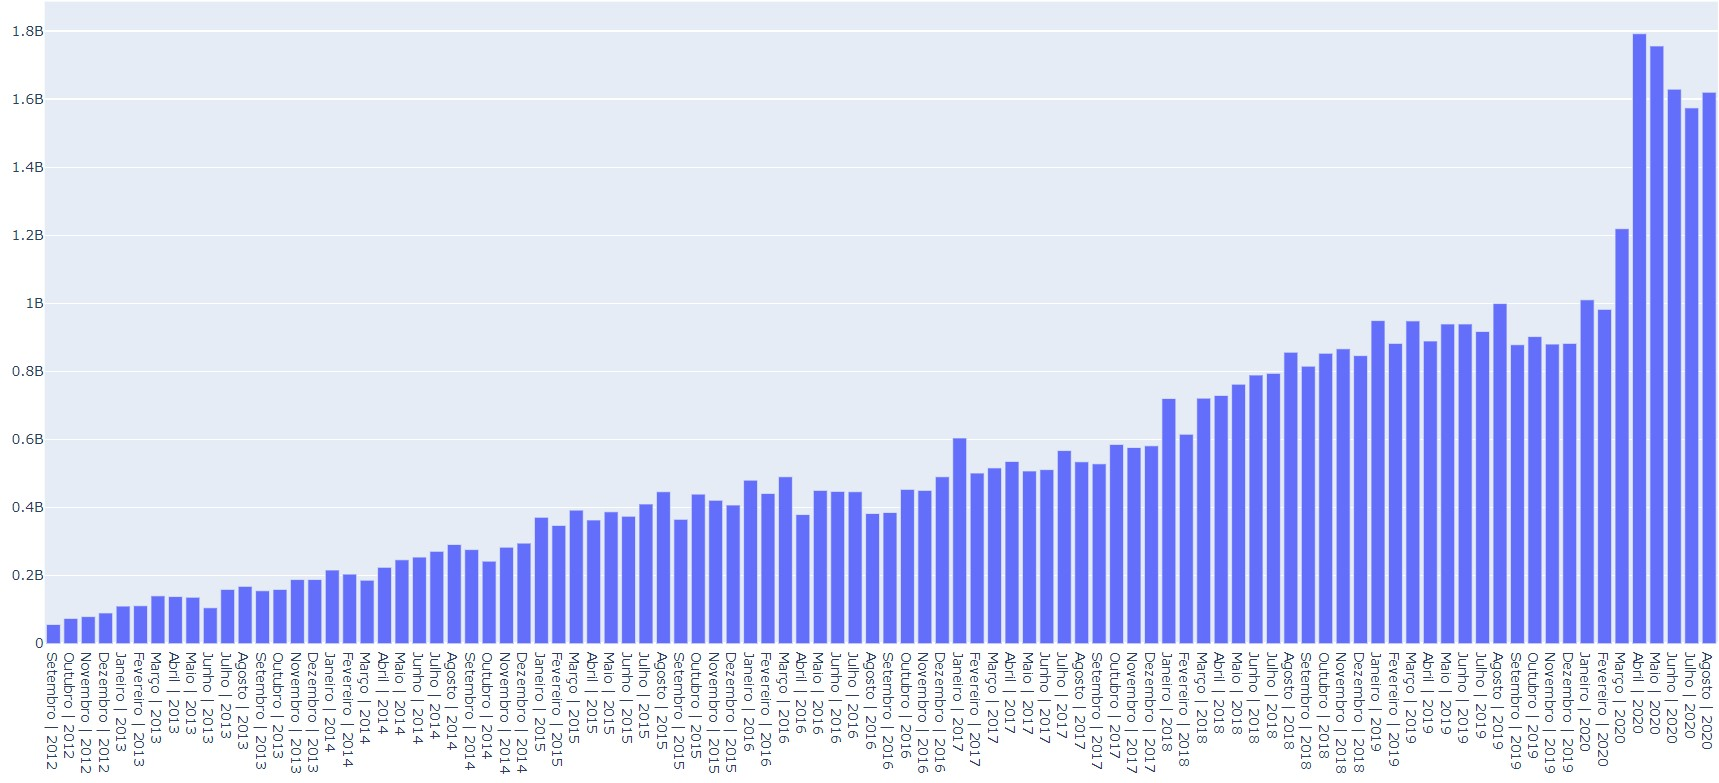
\includegraphics[width=17cm]{Figuras/Tempo_horas.jpg} % leia abaixo
\label{figura:qualquernome}
\end{figure}
Na Fig. \ref{figura:qualquernome}, Grafico em barras do tempo em horas assistido na plataforma
\begin{figure}[h]
\caption{Tempo em horas}
 
\centering % para centralizarmos a figura
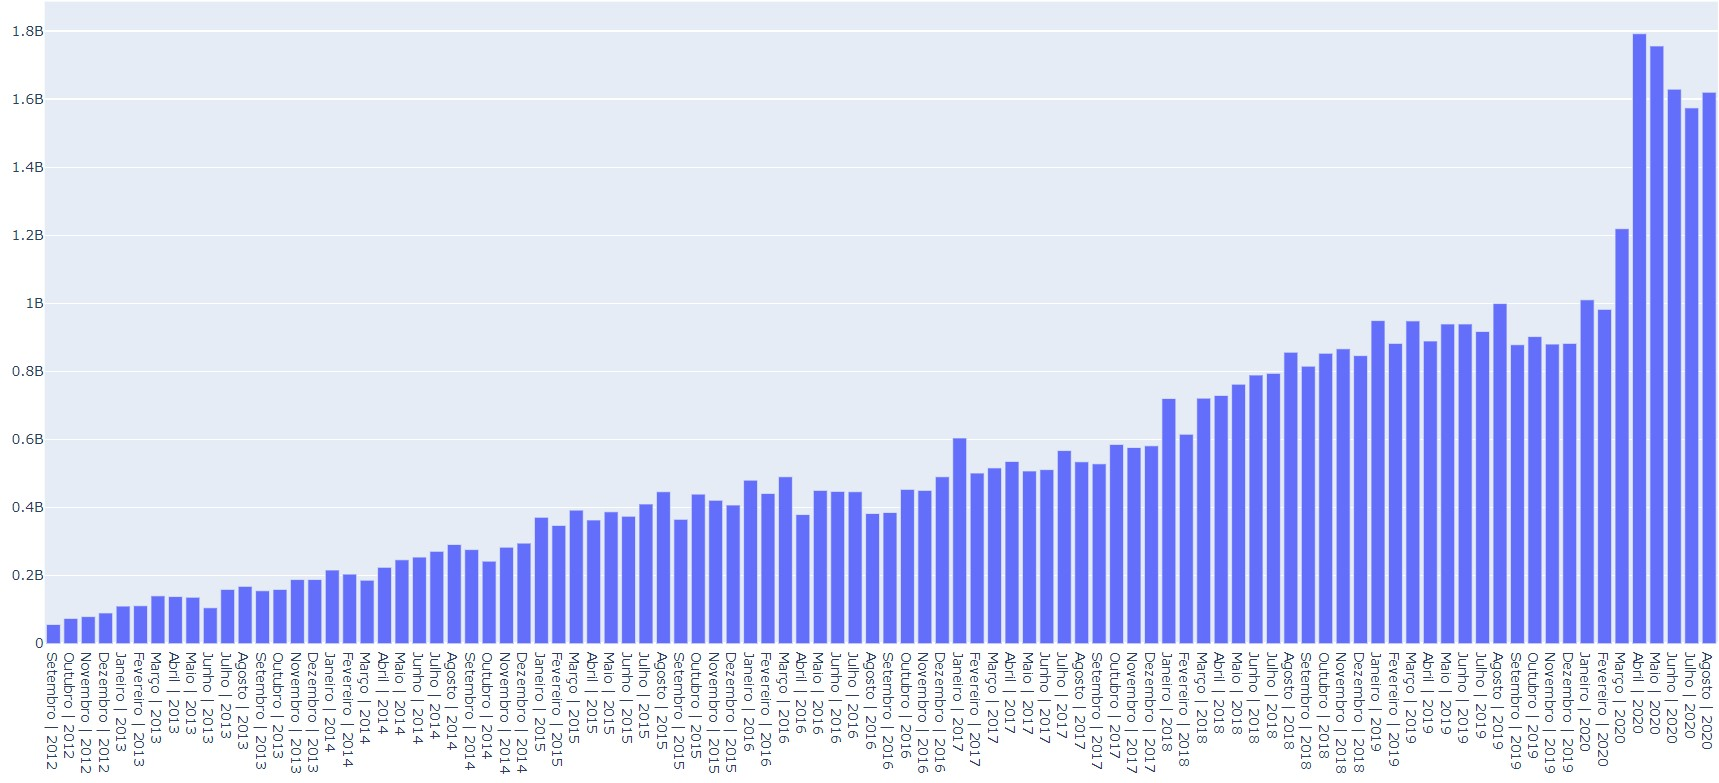
\includegraphics[width=17cm]{Figuras/Tempo_horas.jpg} % leia abaixo
\label{figura:qualquernome}
\end{figure}
Na Fig. \ref{figura:qualquernome}, Grafico em barras do tempo em horas assistido na plataforma

\end{apendicesenv}
